\section{Zielsetzung}
In diesem Versuch soll der
Aufbau eines Helium-Neon-Lasers untersucht werden.
Genauer soll die Stabilitätsbedingung des Lasers überprüft, zwei 
transversal emittierte Moden (TEM-Moden) vermessen, die Polarisation des 
ausgesandten Lichtes gemessen und die Wellenlänge bestimmt werden.

\section{Theorie}
\label{sec:Theorie}

In diesem Versuch wird ein Helium-Neon-Laser (light amplification by stimulated emission 
of radiation) verwendet.

\subsection{Prinzip eines Helium-Neon-Lasers}

Allgemein ist ein Laser aus drei Hauptbestandteilen aufgebaut. Damit sind ein 
verstärkendes Medium, ein Resonationssystem und eine Energiepumpe gemeint.
Das verstärkende Medium ist in diesem Fall das Helium-Neon-Gasgemisch, welches sich 
in einer Glasröhre befindet, an deren Enden sogenannte Brewster-Fenster angebracht sind.
Fällt Licht auf die Brewster-Fenster ein, das parallel zu ihrer Ebene polarisiert ist,
so kann es die Fenster unreflektiert passieren. Restliche Polarisationsrichtungen werden jedoch
zu einem Teil reflektiert. Eine Polarisationsrichtung wird also gegenüber den anderen 
bevorzugt (Mode des Lasers). Hinter den Brewster-Fenstern befinden sich die 
Elemente des Resonators. Es sind zwei Spiegel, die unterschiedlich gewölbt sein können.
Das bedeutet, es handelt sich um einen optischen Resonator, indem sich eine 
stehende Welle durch Interferenz bilden kann, falls die halbe Wellenlänge des Lichtes ein 
Vielfaches der Resonatorlänge ist.\\\\
Generell ist die Wellenlänge des Lasers von den Energieübergängen abhängig, die in ihm 
stattfinden. So gilt für die Frequenz des emittierten Lichtes 
\begin{equation}
    \nu = \frac{ E_{\text{k}} - E_{\text{i}} }{h}.
    \label{eq1}
\end{equation}
In dieser Gleichung beschreibt $E_{\text{k}}$ die Energie des angeregten 
und $E_{\text{i}}$ die Energie des tieferen Zustandes \cite{1}.
Die Wellenlänge $\lambda$ lässt sich dann mittels eines Gitters bestimmen, wobei die 
notwendigen Formeln durch

\begin{equation}
    \varphi_{\text{n}}=\arctan{\left(\frac{b_{\text{n}}}{d}\right)},\qquad \lambda = a\cdot\frac{\sin{\left(\varphi_{\text{n}}\right)}}{\text{n}}
    \label{eq:phi_n}
\end{equation}

gegeben sind. In Gleichung \eqref{eq:phi_n} entspricht $a$ der Gitterperiode, $b_{\text{n}}$ der Position der Beugungsmaxima relativ zum Strahlmittelpunkt und 
$d$ der Distanz zum Schirm, auf den die Maxima porjiziert werden \cite{2}.\\\\
Damit es zu Übergängen dieser Art kommen kann, muss zunächst Energie in das 
System gepumpt werden.
Im Laseraufbau sind dafür zwei Elektroden an den Enden des Glasröhrchens installiert, 
sodass ein Strom von einer Elektrode zur anderen durch das Gas fließen kann.
Dabei wird das Gas, bzw. die Heliumatome ionisiert und angeregt,
sodass es sich auf einem Energieniveau von annähernd gleicher Höhe wie Neon befindet.
Dann können die Heliumatome Stöße zweiter Art mit Neon durchführen.
Das führt zu einer Anregung der Neonatome, sodass von Besetzungsinversion 
gesprochen werden kann. Eine initiale spontane Photonemission eines angeregten 
Neonatoms führt daraufhin zu stimulierter Emission durch weitere angeregte Neonatome. 
Diese Photonen bilden das Laserlicht. Wenn ihre Polarisation nicht durch die 
Brewster-Fenster reflektiert wird, dann werden sie durch die Resonatorspiegel 
immer wieder durch das verstärkende Medium geleitet, woraufhin es zu immer mehr
stimulierter Emission kommt. Schließlich kann der Laserstrahl das System durch einen 
der teildurchlässigen Resonatorspiegel verlassen. Dadurch entsteht jedoch auch ein 
Auskopplungsverlust \cite{2}.\\\\
Der verwendetet Helium-Neon-Laser ist ein Vier-Niveau-Laser, wobei für die 
Energieniveaus gilt: $E_{\text{0}} <E_{\text{1}} < E_{\text{2}} < E_{\text{3}}$.
Bei einem solchen Laser wird von $E_{\text{0}}$ nach $E_{\text{3}}$ gepumpt. 
Außerdem gilt die Bedingung, dass der Übergang von $E_{\text{1}}$ nach $E_{\text{0}}$
durch spontane Emission sehr schnell verläuft, sodass die entsprechenden 
Elektronen schneller wieder auf $E_{\text{3}}$ gepumpt werden, als sie von dort 
aus wieder zurück in den Grundzustand sinken können. Außerdem muss die 
Bedignung gelten, dass der Übergang von $E_{\text{2}}$ nach $E_{\text{1}}$
sehr langsam verläuft. Dann sammeln sich viele Elktronen in $E_{\text{2}}$ \cite{3}.

\subsection{Stabilität eines optischen Resonators}

Allgemein kann zwischen instabilen und stabilen Resonatoren unterschieden werden.
Als stabil gilt ein Resonator genau dann, wenn der Lichtstrahl den Resonator immer
wieder durchläuft und nicht nach einigen Umläufen komplett ausgekoppelt wird.
Stabilität wird dann erreicht wenn die Länge des Resonators einem Vilefachen der 
halben Wellenlänge des Lichtes entspricht. Dann ergibt sich eine stehende Welle,
deren Frequenz anderen Moden gegenüber bevorzugt wird, da sie durch wiederholtes 
Durchlaufen des Mediums weitere Emission dieses Spektrums induziert.
Es wird von gespeicherter Pumpenergie innerhalb dieser Strahlungsenergie gesprochen.
Zur Realisation eines stabilen Resonators muss die Stabilitätsbedingung 
\begin{equation}
    0 < g_1 \cdot g_2 <1 bzw. g_1 = g_2 = 0
    \label{eq3}
\end{equation}
gelten, wobei die Stabilitätsparameter $g_{\text{i}}$ über die Realtion 
\begin{equation}
    g_1 \cdot g_2  = \left( 1- \frac{d}{b_1} \right) \cdot \left(1 - \frac{d}{b_2} \right)
    \label{eq4}
\end{equation}
definiert sind. In Gleichung \eqref{eq4} bezeichnen die Parameter $b_{\text{i}}$ die 
Krümmnugsradien der Resonatorspiegel, wobei auch $b_{\text{i}} = \infty$ gelten kann, 
wenn es sich um einen flachen Spiegel handelt.
$d$ bezeichnet den Abstand zwischen den Spiegeln. 
Das bedeutet Gleichung \eqref{eq4} ist für zwei konkave Spiegel quadratisch in $d$ und 
zeigt für einen flachen und einen konkaven Spiegel eine lineare Abhängigkeit von $d$ \cite{1}.
\begin{figure}
    \centering
    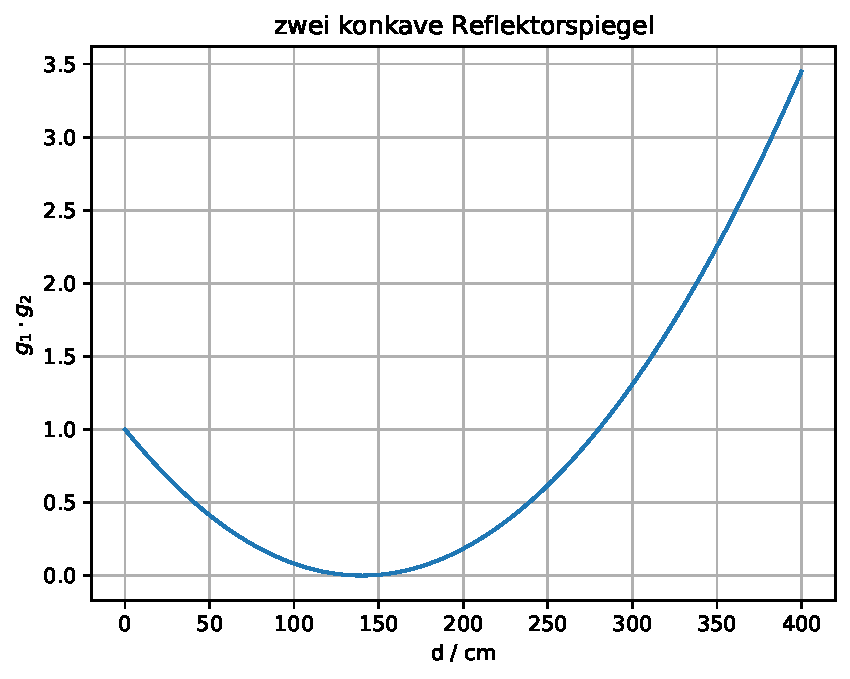
\includegraphics[width=0.6\textwidth]{figure/d_quad.pdf}
    \caption{Auf dieser Abbildung ist der Verlauf von Gleichung \eqref{eq4} 
    dargestellt, wobei für die Parameter $b_{1}=b_{2} = \SI{140}{\centi\meter}$ gilt.}
    \label{abb1}
\end{figure}
\begin{figure}
    \centering
    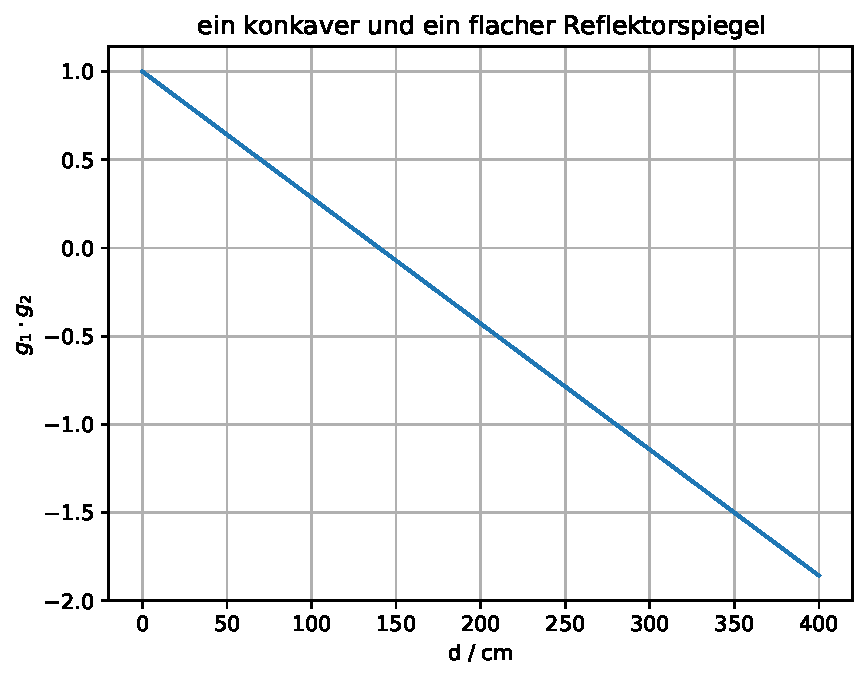
\includegraphics[width=0.6\textwidth]{figure/dlin.pdf}
    \caption{Auf dieser Abbildung ist ebenfalls der Verlauf von Gleichung \eqref{eq4}
    dargestellt, wobei für die Parameter $b_{1} = \infty$ und $b_{2} = \SI{140}{\centi\meter}$ 
    gilt.}
    \label{abb2}
\end{figure}

\subsection{Resonatormoden}

Die Realisation des Lasereraufbaus ermöglicht eine Multimodenstruktur. Das bedeutet 
innerhalb des Resonator überlagern sich mehrere Moden, sogenannte 
$TEM_{\text{mn}}$-Moden. TEM steht für transversale elektromagnetische Mode und die 
Indizes beschreiben die Ordnung der radialen und transversalen Moden.
In Lasern, deren Polarisation durch bspw. Brewster-Fenster linear ist, ergeben sich 
rechtwinklige Moden, wie sie auf Abbildung \ref{abb3} dargestellt sind.
\begin{figure}
    \centering
    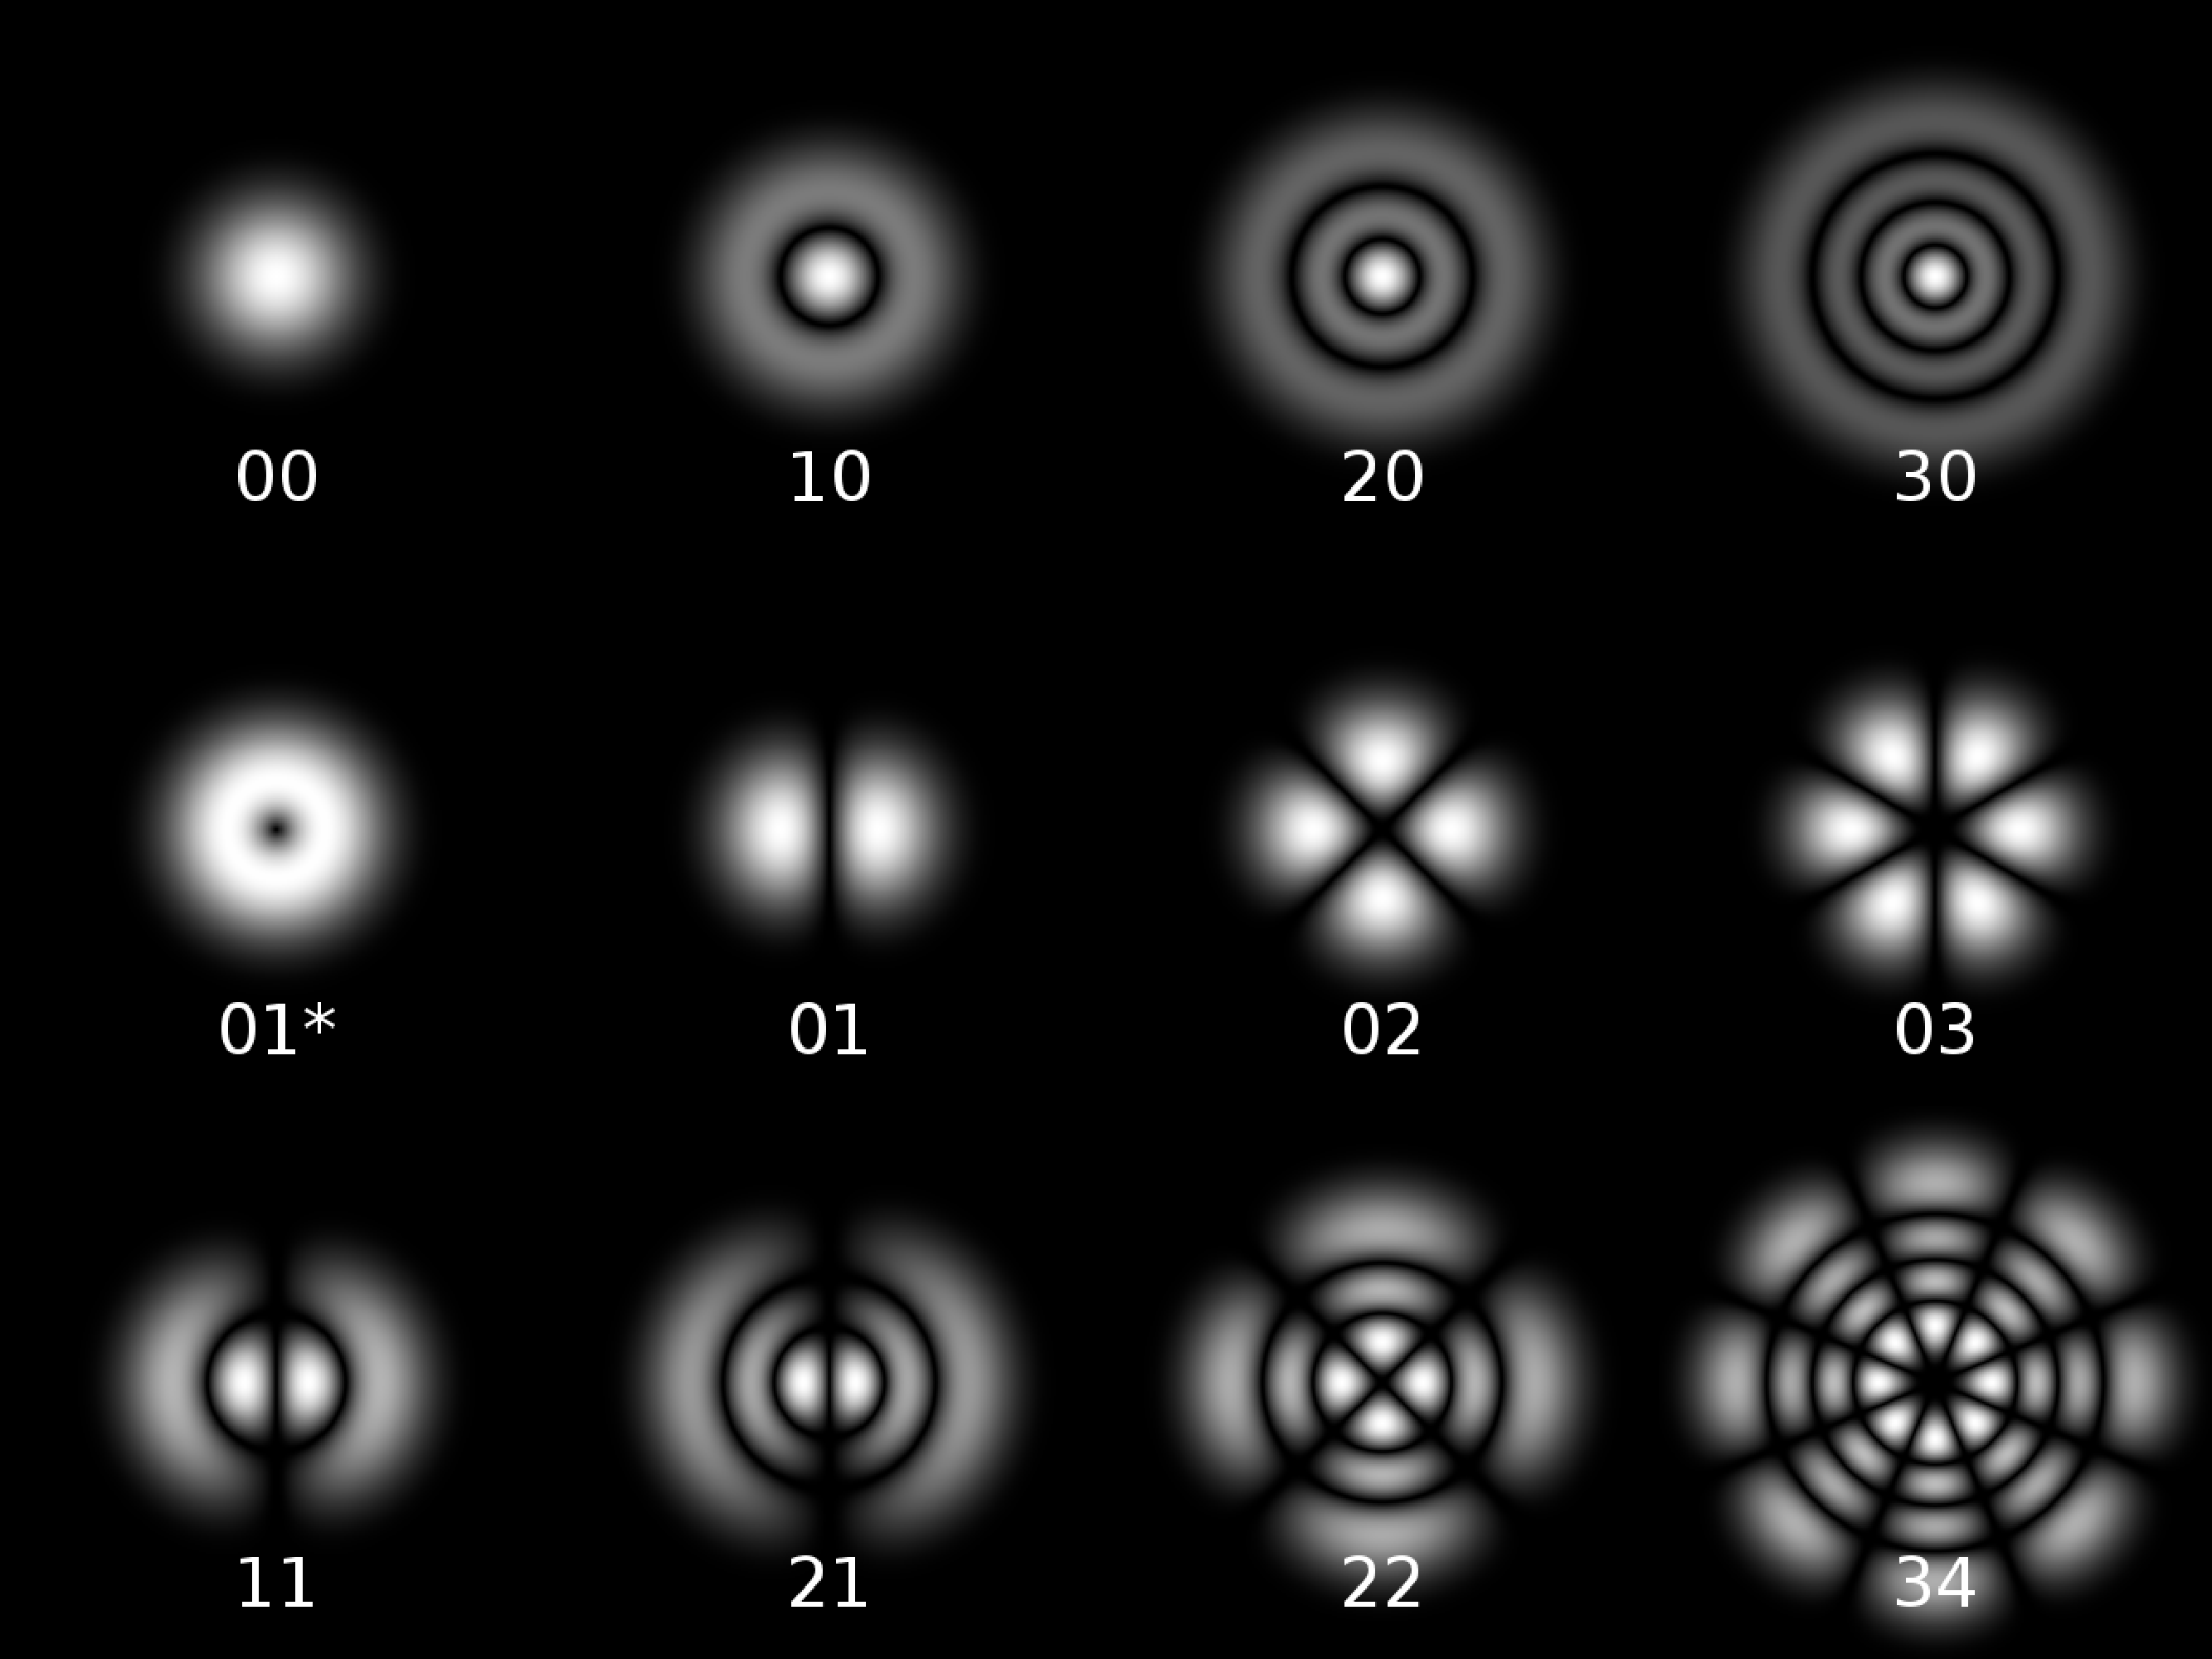
\includegraphics[width=0.6\textwidth]{figure/TEMmoden.pdf}
    \caption{Diese Abbildung zeigt verschiedene rechtwinklige $TEM_{\text{mn}}$-Moden 
    eines Lasers mit Brewster-Fenstern, wie er in diesem Versuch genutzt wurde.
    \cite{TEMmoden}.}
    \label{abb3}
\end{figure}
Ohne selektiv wirkende optische Filterelemente erscheint auf einem Schirm hinter dem 
Ausgang des Lasers immer die $TEM_{\text{00}}$-Mode, da sie eine Überlagerung aller 
Moden darstellt. Mit entsprechenden Modenfiltern 
können diverse Moden herausgefiltert werden, sodass auch andere $TEM_{\text{mn}}$-Moden
dargestellt werden können.
Die Amplitudenverteilung jeder $TEM_{\text{mn}}$-Mode kann über die Formel 
\begin{equation}
    A_{\text{mn}} (x,y,z) = C_{\text{mn}} H_{\text{m}}(x^*) H_{\text{n}}(y^*) \exp(- \frac{x^{*2} + y^{*2}}{ 4} ) \exp(-i\Phi(x,y,z))
    \label{eq5}
\end{equation}
bestimmt werden, wobei $C_{\text{mn}}$ ein Normierungsfaktor, 
$H_{\text{m}}$ und $H_{\text{n}}$ die Hermite-Polynome und $x^*$ und $y^*$ die 
normierten Koordinaten mit $x^* = \sqrt{2}x/\omega$ und 
$y^* = \sqrt{2}x/\omega$ beschreiben. Dabei gilt für $\omega$ die Definition
\begin{equation}
    \omega(z) = \sqrt{ \lambda \frac{d}{2 \pi } \left( 1+ \left( \frac{2z}{d} \right)^2 \right) }
\end{equation}
mit der Wellenlänge $\lambda$. 
Bezüglich der Intensitätsverteilung gilt die Proportionalität
\begin{equation}
    I(x,y) \propto |A_{\text{mn}}|^2
    \label{eq6}
\end{equation} 
\cite{1}.
\newpage
